\section{Lezione 5} \hfill 04/03/2026\\
In area mediterranea esistono ulteriori formazioni, che possono anche esularsi da quelli naturali.
\subsubsection{Sughera - Quercus suber}
Le formazioni di questa specie prendono il nome di sugherete.\\
La Quercia da sughero può ibridarsi con il cerro (Quercus cerris) e dare vita ad una nuova specie.\\
Ha caratteristiche ecologiche simili a quelle del leccio: si trova nello stesso ambiente mediterraneo, ma necessita di migliori condizioni stazionali (ha maggiori esigenze idriche del leccio).\\
Il ritidoma è spesso (corteccia), dal quale si ottiene il sughero. Per questo motivo la sughera è coltivata da migliaia di anni:
\begin{itemize}[nosep]
    \item il materiale è ecologico (non è sintetico);
    \item si presta a tantissimi usi (es. tappi di bottiglie);
    \item è un ottimo isolante termico e sonoro;
    \item brucia in moto limitato, data la presenza di tannini all'interno.
\end{itemize}
In Italia la sughericoltura è svolta soprattutto in Sardegna, ed in minor parte in Sicilia e Toscana.\\
La sughereta è un classico esempio di agroforestazione: per ottenere molto sughero è necessario che gli alberi siano grandi, con larghe  chiome libere: il prodotto finale non dev'essere il legno, bensì il sughero.\\
La sughereta non è un bosco, ma è un'area coperta da alberi isolati (50-70 \unit{n/ha}): in mezzo agli alberi può essere svolto il pascolo, può essere mantenuto il prato oppure possono essere eseguite coltivazioni agrarie.\\
Oggi le produzioni di sughero in Italia sono limitate; il prodotto viene importato dalla Spagna o dal Portogallo.\\
La pianta viene piantata e fatta crescere fino a 2-3 m di toppo (ovvero il fusto principale esente da rami), con una chioma più ampia possibile. Quando raggiunge i 20 cm DBH (occorre una ventina di anni), avviene la demaschiatura: si incide il fusto, non rovinando il cambio, e viene rimossa la corteccia; si ottiene così il sughero maschio, che è inutile e viene buttato (piena d'impurità e buchi). Dopo una decina d'anni viene ripetuta l'operazione, ottenendo così il sughero femmina: ogni decina d'anni verrà così ottenuto sughero.\\
Il legno per i tappi è il sughero più nobile; i sugheri per macerazione sono quelli meno nobili.  
\begin{figure}[htbp]
     \centering
     % Prima Immagine
     \begin{subfigure}[b]{0.33\textwidth}
         \centering
         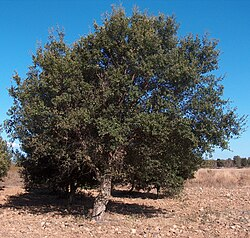
\includegraphics[width=\textwidth]{immagini/quercus_suber_portamento.jpg}
         %\caption{}
     \end{subfigure}
     \hfill % Spazio elastico tra le immagini
     % Seconda Immagine
     \begin{subfigure}[b]{0.3\textwidth}
         \centering
         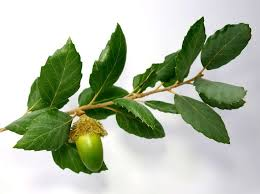
\includegraphics[width=\textwidth]{immagini/quercus_suber_foglie.jpg}
         %\caption{}
     \end{subfigure}
     \hfill % Spazio elastico tra le immagini
     % Terza Immagine
     \begin{subfigure}[b]{0.3\textwidth}
         \centering
         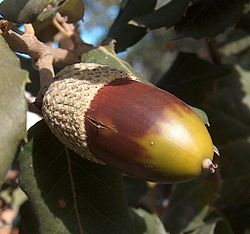
\includegraphics[width=\textwidth]{immagini/quercus_suber_ghiande.jpg}
         %\caption{}
     \end{subfigure}
     
    % \caption{Didascalia generale del gruppo di immagini.}
     \label{fig:quercus_suber}
\end{figure}
\vspace{1cm}
L'ambiente mediterraneo è stato da sempre povero di boschi. Nell'ultimo secolo si è cercato di fare selvicoltura industriale (selvicoltura nel quale il bosco ha la sola funzione di produzione) ed arboricoltura da legno (la produzione di legno è fuori dal bosco, in area agricola). Per fare questo, molto spesso sono state utilizzate specie esotiche. Queste specie possono essere suddivise in due gruppi:
\begin{itemize}[nosep]
    \item latifoglie: solamente eucalipti;
    \item conifere: fondamentalmente il Pinus radiata ed il gruppo di specie Pitch pine 
\end{itemize}
\subsubsection{Eucalipti}
Sono originari dell'Australia, dove sono presenti un centinaio di specie di eucalipti: colonizzano dalle aree costiere fino alle aree di montagna (da situazioni molto secche e calde fino alle situazioni umidi).\\
Gli eucalipti mediterranei crescono bene anche al di fuori delle loro aree di origini, soprattutto se senza competizione. La pianta è idrogora, con un notevole consumo del suolo.\\
Ci sono circa 6-7 specie adatte ai climi mediterranei. Fondamentalmente sono l'Eucalyptus globulus e l'Eucalyptus camaldulensis.\\
In altre parti del mondo ci sono altre specie.\\
Le foglie sono lanciolate, con un aroma tipico ed una formidabile capacità pollonifera caulinare.\\
I giovani polloni hanno foglie completamente diverse che da adulti: con una forma reniforme ed un colore verde glauco, utilizzati per i mazzi di fiori.\\
Il legno di eucalipto è:
\begin{itemize}[nosep]
    \item molto duro e pesante;
    \item peso specifico spesso superiore a 1; 
    \item soffre di forti ritiri tangenziali.
\end{itemize}
La coltivazione dell'eucalipto viene svolta principalmente per la produzione della pasta da carta.\\
In Italia, è stata provata la coltivazione negli anni '50-'60, senza però ottenere successo: il clima richiesto è quello mediterraneo, ma senza la nostra siccità estiva. Oggi è possibile trovarla nei campeggi.\\
Il popolamento può crescere dai 30 ai 60 \unit{m^3/ha \cdot y}.\\
All'estero si trovano impianti artificiali, solitamente con 2 turni: a ciclo breve o a ciclo medio. L'impianto normalmente può essere a 4x3 o 4x4, con 12-15 \unit{m^2} di spazio per singola pianta. I turni sono di 6-7 anni per la produzione di tondelli per la pasta da carta; oppure di 10-15 anni per assortimenti da paleria. Un altro assortimento ricavato da questa pianta è l'eucaliptolo.\\
A fine turno il sistema viene ceduato con una ceduazione semplice (nessuna matricina), e la ceppaia ricaccia.\\
Gli eucalipti sono stati introdotti in molte aree con clima mediterraneo, anche in virtù delle loro rapide crescite: bacino del Mediterraneo, Spagna, Portogallo, Argentina, Cile, Uruguay, Paraguay, Sud Africa, Indonesia, India, Australia, Nuova Zelanda. Per esempio, in Portogallo le temperature sono alte, ma piove: questo è dovuto all'umidità relativa alle correnti umide dell'oceano.\\
Data la grande quantità di cere presenti all'interno dell'albero, quando l'individuo inizia a bruciare, la combustione avviene velocemente.\\
È un enorme consumatore di suoli, portando alla perdita di fertilità.
\begin{figure}[htbp]
     \centering
     % Prima Immagine
     \begin{subfigure}[b]{0.33\textwidth}
         \centering
         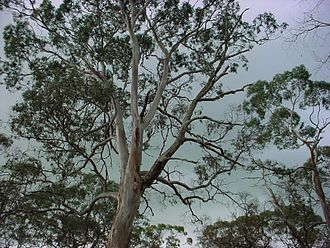
\includegraphics[width=\textwidth]{immagini/eucalipto_portamento.jpg}
         \caption{Portamento.}
     \end{subfigure}
     \hfill % Spazio elastico tra le immagini
     % Seconda Immagine
     \begin{subfigure}[b]{0.3\textwidth}
         \centering
         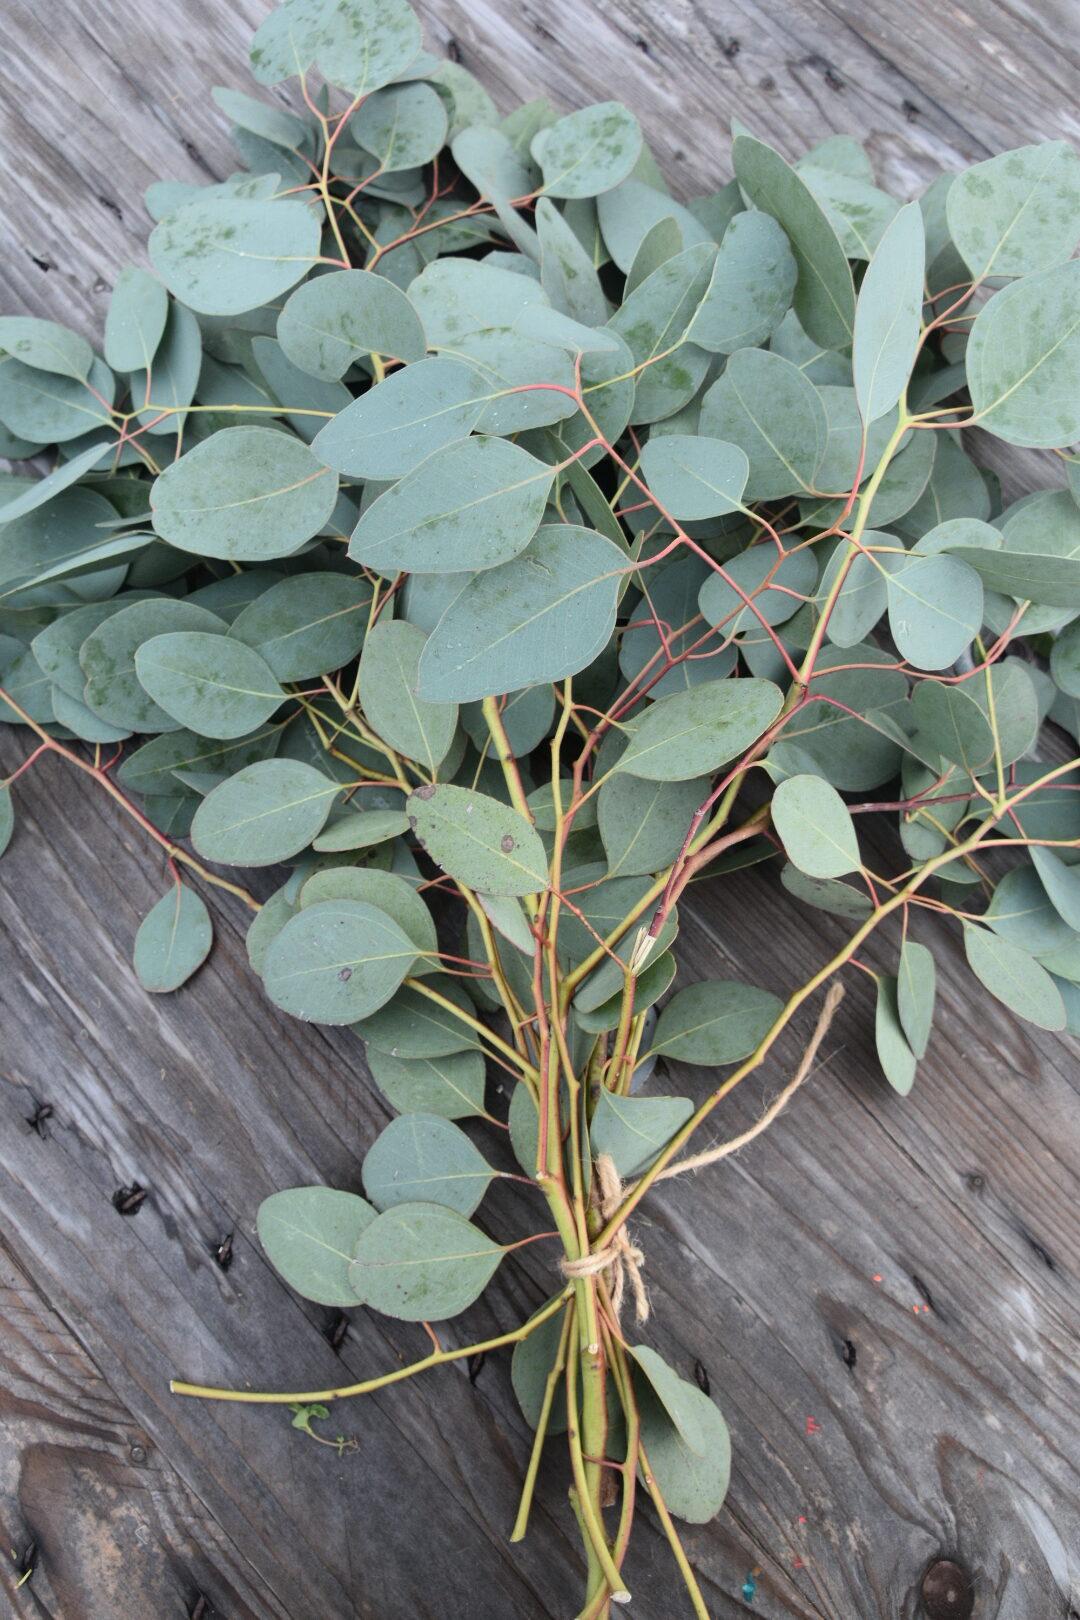
\includegraphics[width=\textwidth]{immagini/eucalipto_foglie_giovani.jpg}
         \caption{Foglie giovani.}
     \end{subfigure}
     \hfill % Spazio elastico tra le immagini
     % Terza Immagine
     \begin{subfigure}[b]{0.33\textwidth}
         \centering
         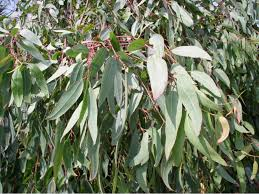
\includegraphics[width=\textwidth]{immagini/eucalipto_foglie_adulte.jpg}
         \caption{Foglie adulte.}
     \end{subfigure}
     
    % \caption{Didascalia generale del gruppo di immagini.}
     \label{fig:eucalipto}
\end{figure}
\subsubsection{Pitch pine}
Insieme di specie di pino: Pinus radiata (Pino radiato), Pinus taeda (Pino taeda), Pinus palustris (Pino palustre), Pinus gountering...\\
Provengono dagli Stati della Carolina, Tennesse., Texas, con un clima simil mediterraneo
\subsubsection{Pino radiato - Pinus radiata}
Anche detto Pino di Monterey, ha un areale ridotto nella California meridionale.\\
È un pino a tre aghi.\\
Gli impianti sono 4x5, 4x4 e 3x6, ed i turni sono intorno ai 24 anni.\\
Gli usi principali sono quelli per la produzione di pasta da carta e tavolami (soprattutto se lavorati). La cellulosa è di qualità migliore rispetto alla cellulosa dell'eucalipto o di latifoglie.\\
È coltivato in tutto l'emisfero australe ed in Sud-Africa.
\begin{figure}[htbp]
     \centering
     % Prima Immagine
     \begin{subfigure}[b]{0.33\textwidth}
         \centering
         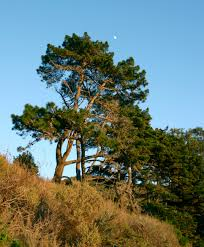
\includegraphics[width=\textwidth]{immagini/pinus_radiata_portamento.jpg}
        % \caption{}
     \end{subfigure}
     \hfill % Spazio elastico tra le immagini
     % Seconda Immagine
     \begin{subfigure}[b]{0.3\textwidth}
         \centering
         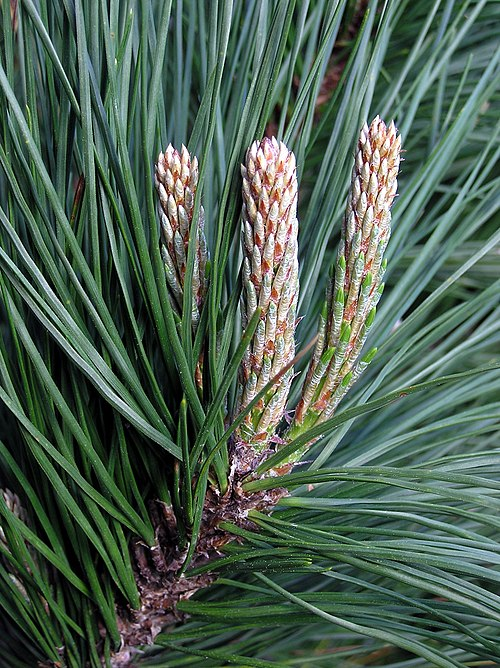
\includegraphics[width=\textwidth]{immagini/pinus_radiata_foglie.jpg}
         %\caption{}
     \end{subfigure}
     \hfill % Spazio elastico tra le immagini
     % Terza Immagine
     \begin{subfigure}[b]{0.33\textwidth}
         \centering
         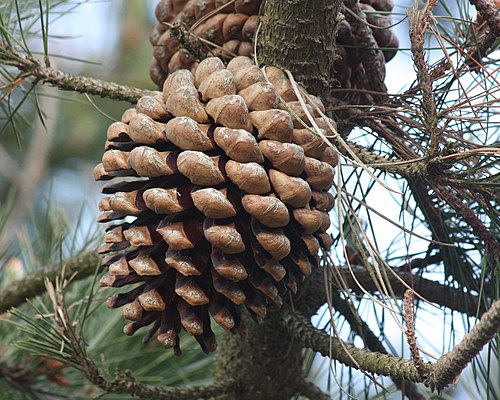
\includegraphics[width=\textwidth]{immagini/pinus_radiata_cono.jpg}
         %\caption{}
     \end{subfigure}
     
    % \caption{Didascalia generale del gruppo di immagini.}
     \label{fig:pinus_radiata}
\end{figure}
\subsection{Pianura Padana}
20000 anni fa la Pianura Padana era un grande mare poco profondo (coda del mare Adriatico). Con il tempo, il Po e gli altri fiumi hanno cominciato a riempirlo (in modo disomogeneo, essendo questi meandriformi), depositando NON suolo (permeabile, tanti ghiaioni).\\
Con il tempo questo materiale è diventato suolo.\\
La pianura è formata da substrati sciolti, fortemente influenzati dall'acqua e dall'uomo.\\
La P.P. era un mosaico di 3 macrostazioni, dando vita a formazioni di tipo diverso: 
\begin{itemize}[nosep]
    \item suoli molto minerali;
    \item suoli fertili e ricchi;
    \item suoli umidi.
\end{itemize}
Con l'arrivo dell'uomo, sono state fatte variazioni sensibili al territorio:
\begin{itemize}[nosep]
    \item taglio di boschi;
    \item bonifiche delle zone umide (es. Polesine, bassa veronese);
    \item irrigazione delle aree secche.
\end{itemize}
Sono rimaste singole isole boscate in P.P. (es. parte del Bosco della Mesola, area del Ticino, Bosco della Partecipanza di Trino, Bosco Fontana nel mantovano).\\
In Veneto c'è un'ottantina di ettari di popolamenti di querco-carpineti.\\
Oggi, l'importanza del bosco planiziale è solamente dal punto di vista ecologico e paesistico-turistico-ricreativo.\\
Ci sono 3 tipi di boschi della P.P. (sub-mediterranea):
\begin{itemize}[nosep]
    \item boschi dei fiumi (formazioni ripariali);
    \item boschi delle aree fertili, senza ristagno idrico, falda freatica poco profonda (sono i querco-carpineti e carpineti);
    \item boschi delle zone umide: alno-unneti.
\end{itemize}
\subsubsection{Anno-unneti}
Sono presenti in vaste aree dell'Unione europea, soprattutto nelle aree dei delta interni dei grandi fiumi.\\
Queste formazioni sono legate alla costante presenza di acqua, possibilmente in lento movimento.\\
In Italia sono quasi scomparse, data le notevoli bonifiche avvenute in passato: sono rimaste solamente in Piemonte e Lombardia (dove i suoli sono ricchi di argilla).
\subsubsection{Olmo - Ulmus}
È la specie dominante della P.P., è scomparso dalla forma arborea, ma sopravvive nella forma arbustiva.\\
Il legno è simile al noce, mediamente duro e versatile.\\
Cresce velocemente.\\
Soffre di grafiosi: è comparsa la prima volta negli anni '80. Uno scolitide entra nella corteccia (sufficientemente spessa, 15-16 cm DBH), fa entrare un fungo che attacca il cambio e porta alla morte dell'albero. Attacca gli alberi di grandi dimensioni.\\
Fruttifica già a 3 anni d'età.\\
Si ibrida molto facilmente con gli olmi esotici (Ulmus pumila, Ulmus laevis), che sono resistenti alla grafiosi.
\begin{figure}[htbp]
     \centering
     % Prima Immagine
     \begin{subfigure}[b]{0.33\textwidth}
         \centering
         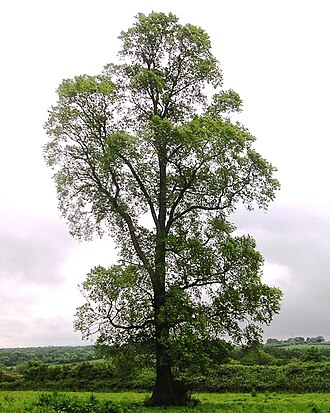
\includegraphics[width=\textwidth]{immagini/ulmus_portamento.jpg}
        % \caption{}
     \end{subfigure}
     \hfill % Spazio elastico tra le immagini
     % Seconda Immagine
     \begin{subfigure}[b]{0.3\textwidth}
         \centering
         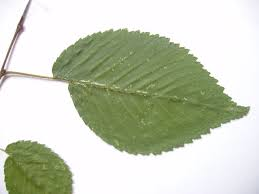
\includegraphics[width=\textwidth]{immagini/ulmus_foglie.jpg}
         \caption{Foglia asimmetrica.}
     \end{subfigure}
     \hfill % Spazio elastico tra le immagini
     % Terza Immagine
     \begin{subfigure}[b]{0.33\textwidth}
         \centering
         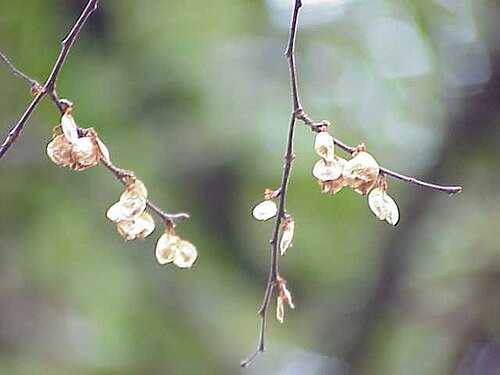
\includegraphics[width=\textwidth]{immagini/ulmus_frutti.jpg}
         %\caption{}
     \end{subfigure}
     
    % \caption{Didascalia generale del gruppo di immagini.}
     \label{fig:ulmus}
\end{figure}
\subsubsection{Ontano - Alnus}
Gli ontaneti sono classiche formazioni azonali (non sono legati ad un certo tipo di clima, ma sono legati ad un certo tipo di suolo).\\
In Nord Italia ci sono 3 (+1) tipi di ontani:
\begin{itemize}[nosep]
    \item ontano nero (Alnus glutinosa): foglie a forma di cuore e glutinoso in primavera;
    \item ontano bianco (Alnus incana): area montana;
    \item ontano verde (Alnus viridis): del piano subalpino;
    \item ontano napoletano (Alnus cordata): dell'area appenninica.
\end{itemize}
Queste specie richiedono molta umidità; è comune trovarli in prossimità di canali o fossature.\\
L'ontano nero ha una forte capacità pollonifera caulinare.\\
Il suo legno:
\begin{itemize}[nosep]
    \item è usato come legna da ardere, poichè non scoppietta;
    \item è morbido ed elastico (usato per oggettistica e giocattoli);
    \item in passato veniva usato come forma dai battilastra;
    \item è pessimo per i pavimenti.
\end{itemize}
È la latifoglia che possiede la forma più simile ad una conifera (monopodiale con leggere ramificazioni laterali): il fusto è di grosse dimensioni, con poca chioma.\\
In Italia viene solitamente gestito a ceduo (capacità pollonifera caulinare), turni di 15-20 anni, spesso con ceduo semplice.\\
Essendo una betulacea, può creare irritazioni allergeniche (da evitare quindi le piantumazioni vicino alle case).\\
In altre zone d'Europa (es. Germania Est, Repubblica Ceca) dove ci sono grandi fiumi (e delta interni), viene gestito a fustaia, con rinnovazione artificiale posticipata (dopo il taglio di rinnovazione).\\
Viene piantato con turni sui 30-40 anni, di difficile gestione pratica, perchè l'area è paludosa e stagnante. Le utilizzazioni sono fatte d'inverno, mediante gru a cavo orizzontali.\\
La richiesta di grandi volumi legnosi riguarda l'importazione dall'estero.
\begin{figure}[htbp]
     \centering
     % Prima Immagine
     \begin{subfigure}[b]{0.33\textwidth}
         \centering
         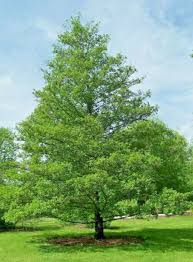
\includegraphics[width=\textwidth]{immagini/alnus_portamento.jpg}
        % \caption{}
     \end{subfigure}
     \hfill % Spazio elastico tra le immagini
     % Seconda Immagine
     \begin{subfigure}[b]{0.3\textwidth}
         \centering
         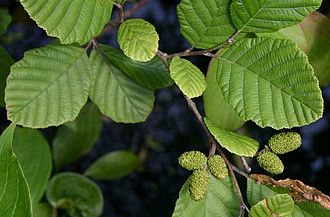
\includegraphics[width=\textwidth]{immagini/alnus_foglie.jpg}
         %\caption{}
     \end{subfigure}
     \hfill % Spazio elastico tra le immagini
     % Terza Immagine
     \begin{subfigure}[b]{0.33\textwidth}
         \centering
         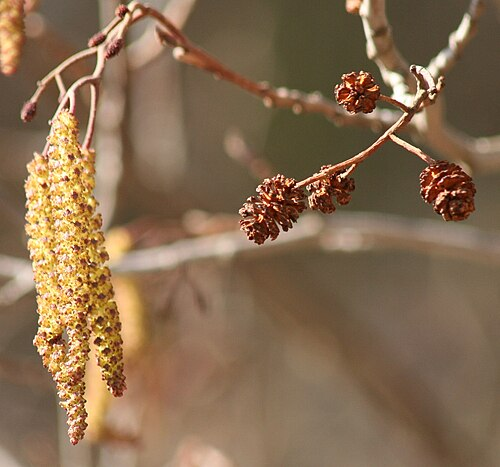
\includegraphics[width=\textwidth]{immagini/alnus_frutti.jpg}
         %\caption{}
     \end{subfigure}
     
    % \caption{Didascalia generale del gruppo di immagini.}
     \label{fig:alnus}
\end{figure}